\documentclass{article}
\usepackage{mathtools}
\usepackage{amssymb}
\usepackage{listings,xcolor}
\usepackage{physics}

\lstset{language=Mathematica}
\lstset{basicstyle={\sffamily\footnotesize},
  numbers=left,
  numberstyle=\tiny\color{gray},
  numbersep=5pt,
  breaklines=true,
  captionpos={t},
  frame={lines},
  rulecolor=\color{black},
  framerule=0.5pt,
  columns=flexible,
  tabsize=2
}

\begin{document}
\title{On the Distribution of $Z\sim\chi^2_{df} + \text{Lap}(b)$}
\author{Mark Schultz}
\maketitle

When discussion a differentially private form of ANOVA, we looked into the following random variable:
\begin{equation}
\widehat{F}\sim \frac{U_1+\text{Lap}(b_1)}{U_2+\text{Lap}(b_2)}
\end{equation}
Here, $U_1$ and $U_2$ are both $\chi^2_{df}$ for some parameter $df$.
The first step to understanding this random variable would be understanding the distribution of $U+\text{Lap}(b)$ for $U\sim\chi^2_{df}$.
Does this potentially have a ``nice'' distribution?

The answer to this is both yes and no --- it has an \emph{explicitly computable} density function (without resorting to things like various special functions such as the hypergeometric function, Meijer G function, or Fox H function).
We can easily\footnote{Given access to a tool that's good at Symbolic Integration, such as \emph{Mathematica}.} \emph{algorithmically} compute this distribution, which will be detailed below.
\section{Sums of independent variables via Moment Generating Functions}
We've so far seen multiple ways to compute to compute the pdf of a random variable.
One of the ``most powerful'' is that of the \emph{moment generating function}, which is defined as:
\begin{equation}
m_X(t) = \mathbb{E}[e^{tX}] = \int_{x = -\infty}^\infty e^{tx}\rho_X(x)\mathrm{ d}x
\end{equation}
Much of the power of this method lies in its close connection to the \emph{Laplace Transform}.
This shares many desirable theoretical properties with the \emph{Fourier Transform}\footnote{In fact, the \emph{characteristic function} $\varphi_X(t) = \mathbb{E}[e^{itX}]$ is defined precisely in terms of the Fourier transform.
This is a complex-valued function though, so is at least a \emph{little} worse to work with numerically.
The benefit is that it always exists, unlike the mgf.}, so one can think of them as roughly equivalent if you want to.
The two main properties we've seen so far are:
\begin{itemize}
\item The Fourier/Laplace Transform take the \emph{convolution product} to the standard product (multiplication).
Specifically, if we define:
\begin{equation}
(f\ast g)(x) = \int_{-\infty}^\infty f(y)g(x-y)\mathrm{ d}x
\end{equation}
Then it follows that:
\begin{equation}
\mathcal{F}[f\ast g](x) = \mathcal{F}[f](x)\mathcal{F}[g](x)
\end{equation}
where $\mathcal{F}[f](x)$ is the Fourier transform (or Laplace transform) of $f$ evaluated at $x$.
\item 
There is a unique correspondence between $f(x)$ and $\mathcal{F}[f](x)$.
In terms of probability theory, either of the characteristic function, or the mgf \emph{uniquely} determine the pdf\footnote{Provided they exist, which the mgf doesn't always}.
\end{itemize}
One property we \emph{haven't} discussed is known as \emph{Fourier Inversion}.
This is just the fact than Fourier-like transforms have easily computable \emph{inverse} transforms.
Unfortunately, this ``easy computation'' can require a certain amount of complex analysis to define, so will be omitted from this writeup.

Fortunately, \emph{Mathematica} has a function:
\begin{center}
\begin{lstlisting}[language=Mathematica]
InverseLaplaceTransform[f(s), s, t]
\end{lstlisting}
\end{center}
This \emph{essentially} computes precisely what we need, and allows us to ``invert'' mgfs.
As a result, we can look up the (known) mgfs for $X\sim\text{Lap}(b)$ and $Y\sim\chi^2_{df}$.
It's then quite easy to compute $m_{X+Y}(t) = m_X(t)m_Y(t)$, which we can then invert.
This can easily be done in \emph{Mathematica}, which the .nb file in this directory includes code for.

This allows us to describe the distribution of $\text{Lap}(b) + \chi^2_{df}$, which Mathematica outputs as:
\begin{center}
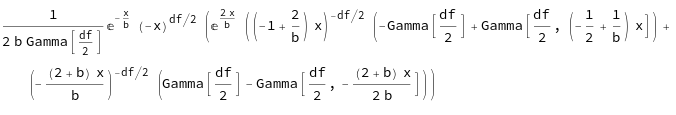
\includegraphics[scale=.5]{distribution.png}
\end{center}
Note here that this includes both $\Gamma(a)$, and $\Gamma(a,x)$.
Here, $\Gamma(a,x)$ is the \emph{incomplete} Gamma function, defined as:
\begin{equation}
\Gamma(a,x) = \int_x^\infty t^{s-1}e^{-t}\mathrm{ d}t
\end{equation}
Note that $\Gamma(a,0) = \Gamma(a)$, so the traditional gamma function is a special case of this.

We can transcribe this into \LaTeX, to get that:
\begin{align*}
\rho_{X+Y}(x) &= \frac{1}{2b\Gamma(df/2)}e^{-x/b}(-x)^{df/2} \\
&\times \left[e^{2x/b}\pqty{\pqty{-1 + \frac{2}{b}}x}^{-df/2}\pqty{-\Gamma(df/2) + \Gamma(df/2, (-(1/2) + (1/b))x)}\right. \\
&\left.+ \pqty{- \frac{(2+b)x}{b}}^{-df/2}\pqty{\Gamma(df/2)-\Gamma(df/2,-\frac{(2+b)x}{2b})}\right]
\end{align*}
We can now try to clean this up some.
To do this, we'll note that it's basic structure has three parts:
\begin{equation}
\rho_{X+Y}(x) = A(B+C)
\end{equation}
where:
\begin{align*}
A & = \frac{1}{2b\Gamma(df/2)}e^{-x/b}(-x)^{df/2} \\
B & = e^{2x/b}\pqty{\pqty{-1 + \frac{2}{b}}x}^{-df/2}\pqty{-\Gamma(df/2) + \Gamma(df/2, (-(1/2) + (1/b))x)} \\
C &= \pqty{- \frac{(2+b)x}{b}}^{-df/2}\pqty{\Gamma(df/2)-\Gamma(df/2,-\frac{(2+b)x}{2b})}
\end{align*}
Note that:
\begin{equation}
\pqty{\pqty{-1 + \frac{2}{b}}x}^{-df/2} = \pqty{-\frac{b-2}{b}x}^{-df/2}
\end{equation}
We additionally have that:
\begin{equation}
\pqty{-\frac{(2+b)x}{b}}^{-df/2} = \pqty{-\frac{b+2}{b}x}^{-df/2}
\end{equation}
We can next look at the (other) factor of each term, which is of the form:
\begin{equation}
\pm\pqty{\Gamma(df/2) - \Gamma(df/2, a)}
\end{equation}
for some $a$.
First, note that:
\begin{equation}
\Gamma(a) - \Gamma(a,x) = \int_0^\infty t^{a-1}e^{-t}\mathrm{ d}t - \int_x^\infty t^{a-1}e^{-t}\mathrm{ d}t = \int_0^x t^{a-1}e^{-t}\mathrm{ d}t = \gamma(a,x)
\end{equation}
Here, $\gamma(a,x)$ is the \emph{lower} incomplete Gamma function.

We have that the first of these $a$ values will be:
\begin{equation}
a = \pqty{-\frac{1}{2} + \frac{1}{b}}x = -\frac{b-2}{2b}x
\end{equation}
It follows that:
\begin{equation}
\Gamma(df/2) - \Gamma(df/2, -\frac{b-2}{2b}x) = \gamma(df/2, -\frac{b-2}{2b}x)
\end{equation}
The other value will be:
\begin{equation}
\gamma(df/2, -\frac{b+2}{2b}x)
\end{equation}
We can therefore try to rewrite the entire pdf, to get that:
\begin{align*}
\rho_{X+Y}(x) &=\frac{1}{2b\Gamma(df/2)}e^{-x/b}(-x)^{df/2}\left(-e^{2x/b}\pqty{\frac{b}{(b-2)(-x)}}^{df/2}\gamma(df/2, -\frac{b-2}{2b}x)\right. \\
&+\left.\pqty{\frac{b}{(2+b)(-x)}}^{df/2}\gamma(df/2,-\frac{(2+b)x}{2b})\right) \\
&=\frac{b^{(df/2)-1}}{2\Gamma(df/2)}e^{-x/b}\pqty{\frac{-e^{2x/b}}{(b-2)^{df/2}}\gamma(df/2, -\frac{b-2}{2b}x)+\frac{1}{(2+b)^{df/2}}\gamma(df/2,-\frac{(b+2)x}{2b})} \\
&=\frac{b^{(df/2)-1}}{2\Gamma(df/2)(b^2-4)^{df/2}}e^{-x/b}\left((b-2)^{df/2}\gamma\pqty{df/2,-\frac{(b+2)x}{2b}}\right. \\
&\left.-e^{2x/b}(b+2)^{df/2}\gamma\pqty{df/2, -\frac{b-2}{2b}x}\right)
\end{align*}
At this point, it's unclear if further simplification is possible.
\end{document}